\chapter{Introduction to Vehicle Routing Problem}\label{introduction_vrp}

    The problem objective of \gls{vrp} is simply finding the shortest route for multiple vehicles to serve all the given set of customers. The shortest route can be differently interpreted based on your minimalization criteria, e.g, traveled distance, time, or a combination of both. It was first proposed by Dantzig and Ramser \cite{truck-dispatching-problem} in 1959, and since then researchers are coming up with different approaches how to solve the problem. 

    \section{Vehicle Routing Problem Definition}
    
    The general \gls{vrp} can be defined as a problem in a complete graph $G=(V,E)$ of finding the optimal permutation $\pi_l = (\pi_0, \cdots, \pi_m)$ of nodes $V$ all starting from a node $v_0$ for given number of paths $k$ which results in minimal traversal cost where $\forall v \in (V \setminus v_0)$ are visited only once. \gls{vrp} is generalization of \gls{tsp} which only has one path.
    
    \begin{figure}[ht]
        \centering
        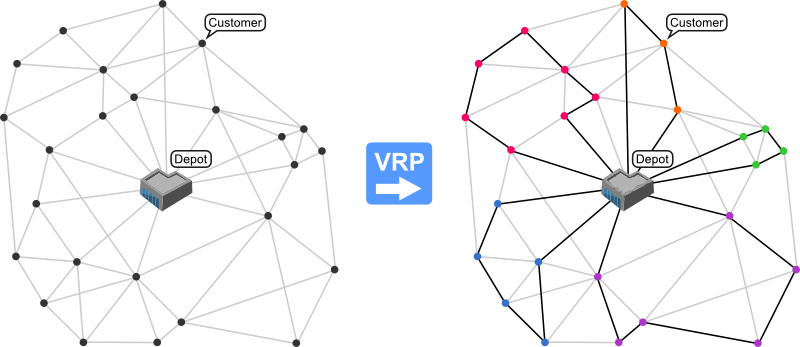
\includegraphics[width=0.75\textwidth]{resources/intro/vrp-graph.png}
        \caption{Intuitive view of \gls{vrp} instance on left and proposed solution for 5 vehicles on the right \cite{vrp-malaga}}
        \label{fig:vrp-graph}
    \end{figure}
    
    \gls{vrp}s are classified as NP-Hard problems which was proved by Lenstra and Kan \cite{time-complexity-vrp}. It means that in the worst case, adding new nodes, i.e., customers results in an exponential increase of computational complexity.
    
    \subsection{VRP Notation}
    Let's introduce our used notation and its real-world interpretation.
    \begin{itemize}
        \item $G=(V,E)$ is a complete undirected graph
        \begin{itemize}
            \item Network of routes
        \end{itemize}
        \item $v_0$ is the initial node
        \begin{itemize}
            \item A depot
        \end{itemize}
        \item $V^{\prime} = (v_1, \cdots, v_n)$ nodes expect the initial node
        \begin{itemize}
            \item Geographically scattered location of customers
        \end{itemize}
        \item $E = \{(v_i, v_j)| v_i, v_j \in V, i \neq j\}$ with associated weight as a cost $c: E \to \mathbb{N}^+$
        \begin{itemize}
            \item A single route between two locations with associated cost, e.g., distance.
        \end{itemize}
        \item $C$ is a matrix of edge weights indexed by nodes. $c_i_j$ where $i,j \in V$
        \begin{itemize}
            \item Matrix of costs between customers
        \end{itemize}
        \item $R_i \subset V$ is a path that starts and ends at $v_0$. $(r_0 = v_0 \land r_{|R_i|} = v_0)$
        \begin{itemize}
            \item Route visit a subset of customers starting and ending at the depot, it can be referred to it as a delivery plan.
        \end{itemize}
        \item $k$ number of paths
        \begin{itemize}
            \item Number of vehicles
        \end{itemize}
        \item $R = R_1, \cdots, R_k$ is a set of paths
        \begin{itemize}
            \item All routes (delivery plans) for a given instance of \gls{vrp}.
        \end{itemize}
        \item $\pi = (\pi_1, \cdots, \pi_k)$ solution for a given instance of \gls{vrp}.
        \begin{itemize}
            \item Customer locations in visiting order for multiple vehicles.
        \end{itemize}
    \end{itemize}
    
    \textbf{Fesability of \gls{vrp} solution} for \gls{vrp} of routes $R$ is feasible only if each node $V_1$ is visited exactly once.
    
    \textbf{The cost of route $R_i$} which we aim to minimize is the sum of its weights (costs). If we operate in Euclidean space, then it is L2 norm of route locations.
    \begin{equation}
        C(R_i) := \sum_{k = 0}^{|R_i|} c_{r_k}_{r_k+1}
    \end{equation}
    
    \textbf{The cost of \gls{vrp} solution} is the sum of route costs.
    \begin{equation}
        C(R) := \sum_{i = 1}^{|R|} C(R_i)
    \end{equation}
    
\section{Vehicle Routing Flavors}
Our modern world heavily relies on complex logistics networks. It requires to synchronize multimodal planning to ship your goods from one side of the world to your doorstep. In order to achieve this, multiple variants and flavours of \gls{vrp} had to be studied and implemented in the real world use cases. It goes from ordinary variants like measuring the capacity of cars to a more niche problem like eVRP where vehicles are required to make stops to recharge.

All the flavours of \gls{vrp} can be mutually combined, which is usually the main area of research.

    \begin{figure}[ht]
        \centering
        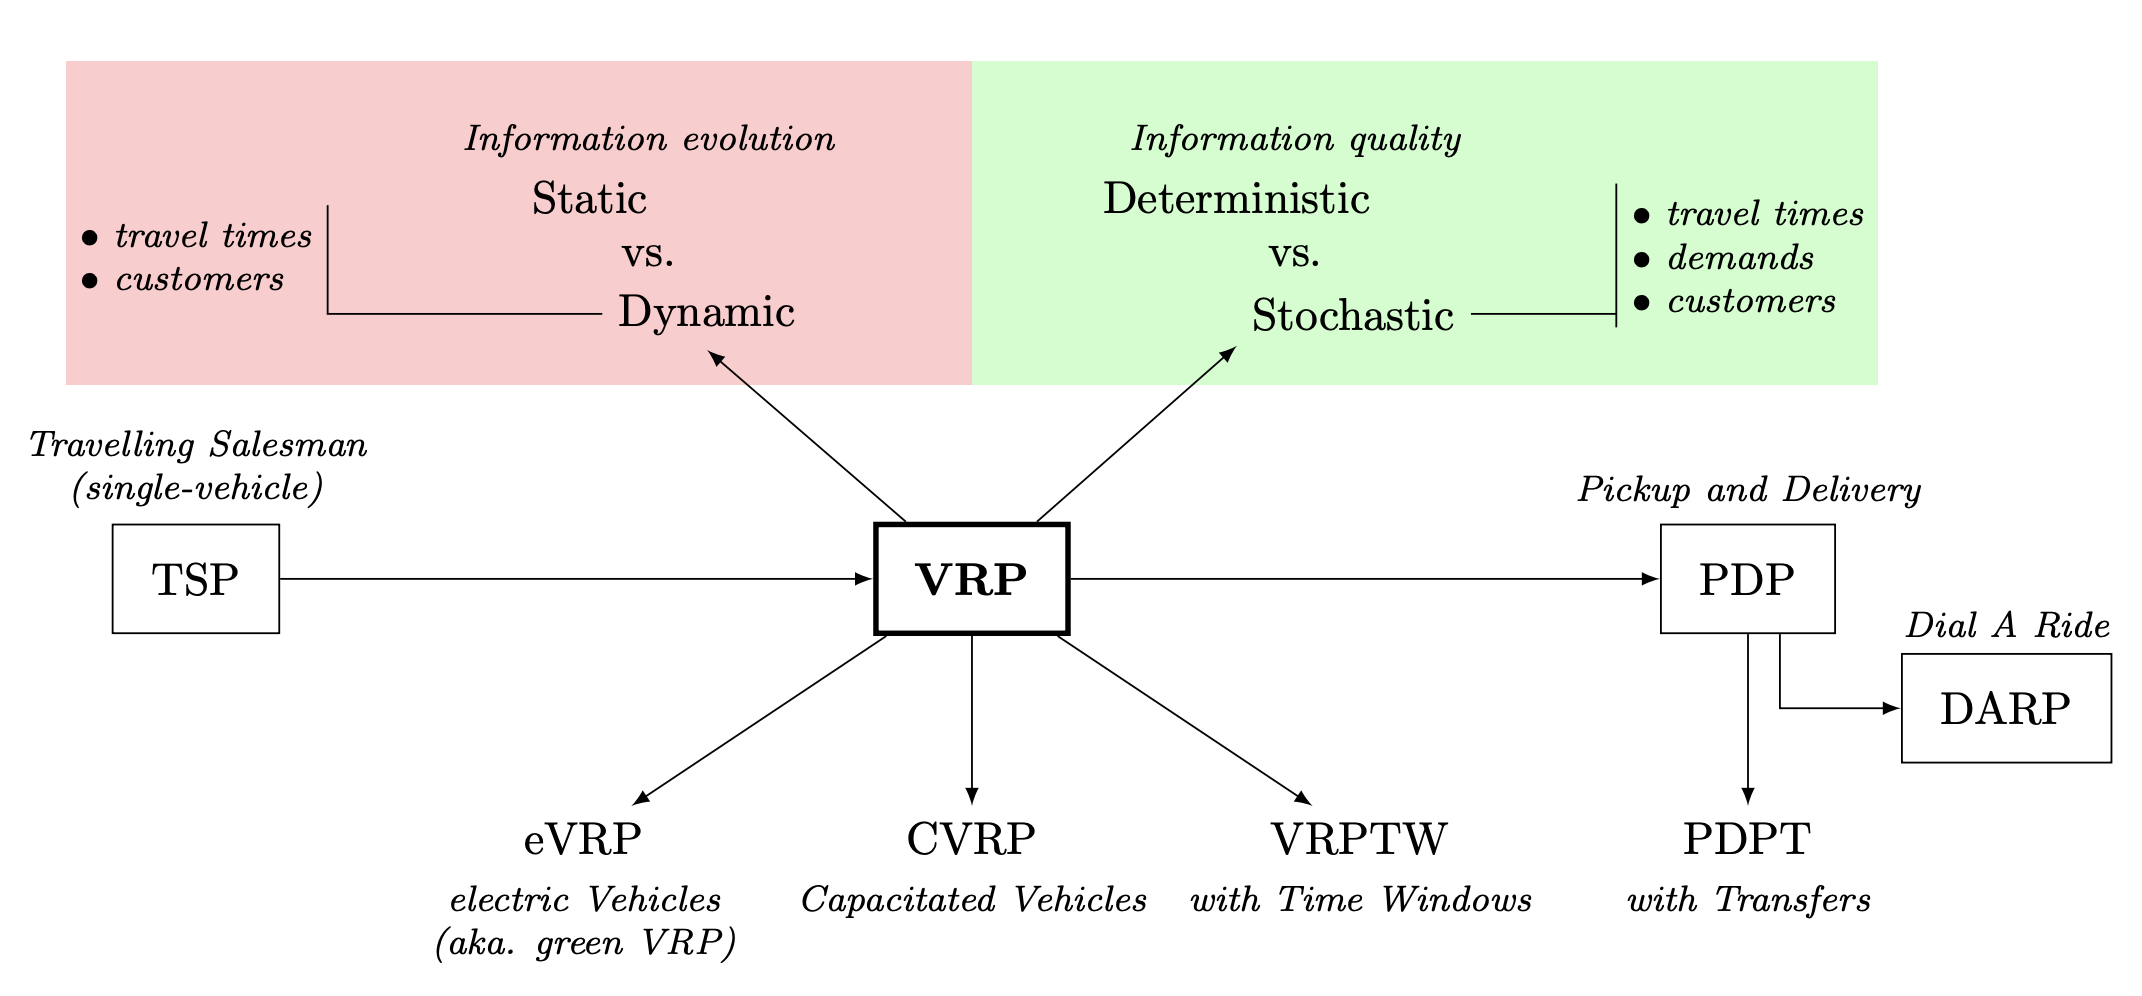
\includegraphics[width=1.0\textwidth]{resources/intro/vrp-flavours.png}
        \caption{Taxonomy of VRPs \cite{bono-stochastic-vrp}}
        \label{fig:vrp-flavours}
    \end{figure}

The sections below are describing each flavour shown in \ref{fig:vrp-flavours}.

    \subsection{Capacitated Vehicle Routing Problem}
    The \gls{cvrp} extends the regular \gls{cvrp} in introducing a capacity element for each customer. In the literature, it is sometimes referred to as a demand. The customer's demand is $d \in \mathbb{N}^+$ which may represent capacity in the form of weight, size but also in some abstract concepts such as a basket of apples. Additionally, each vehicle has a predefined capacity $Q > 0$.
    
    The \gls{cvrp} extends the solution feasibility formula by the following capacity constrain.
    \begin{equation}
        q(R) := \sum_{i \in R} d_i \leq Q
    \end{equation}
    
    If the vehicle capacity of the fleet stays the same, we are dealing with \gls{cvrp} with homogeneous fleet. A fleet with varying capacity for each vehicle is a heterogeneous fleet.
    
    \subsection{Vehicle Routing Problem with Time Windows}
    The \gls{vrptw} \cite{vrptw-solomon} extends the regular \gls{vrp} by time constraint for each customer. Customers have assigned time window interval $[e_i, l_i]$ where $e_li < l_i$. The time interval is the request within a vehicle is supposed to visit the node. 
    
    The time window can be either implemented as a hard constraint or a soft constraint. Hard constraint forces the vehicle to visit the node, i.e., the customer either in the given time interval or the solution is not feasible. Soft constrains are not strictly enforcing the vehicle to visit the customer, but they introduce a penalty for a violated interval barring a penalty cost. The penalty becomes a part of the cost function which \gls{vrp} aims to minimize.
    
    In this thesis, we will be focusing on soft constraints for time windows since it is a better reflection of real world use cases. Most businesses allow couriers to arrive late or early, but these types of arrivals are supposed to be minimized.
    
    \subsection{Pick and Deliver}\label{pick-and-delivery}
    The \gls{pdp} extends the regular \gls{vrp} by pairing pick and drop with precedence relationships, in which a pickup point must precede the paired delivery point. This flavour of \gls{vrp} is one of the most complex and even challenging for conventional methods like optimization heuristics algorithms.
    
    The feasibility of a \gls{pdp} solution is checking whether all delivery points have preceded pickup point.
    
    \subsection{Static vs. Dynamic}\label{dynamic}
    When solving the vehicle routing model, usually we assume that all the input data are static and known with certainty. However, this is not the case in real-life applications where data such as customer demand or travel time are often incomplete or not precise during the planning phase, they are only gradually revealed and specified.
    
    \textbf{Static \gls{vrp}} does not assume that the input data could be subject to change. The \textbf{dynamic \gls{vrp}} is aware about the information evolution\cite{psaraftis} and its goal is to obtain a robust routing planner that will be able to solve already seen instance with subject to small changes without need of recalculating the whole instance again. This is called a priori optimization, after solving a given instance of a combinatorial optimization problem, it becomes necessary to repeatedly solve many other instances with a small variation from the original instance but without reconsideration of the entire problem \cite{apriori-optimization}.
    
    In this thesis, the \gls{vrp} based on \gls{ai} could be a great candidate for dynamic \gls{vrp} even though, the entire instance is being recalculated. The reason is that the problem solution is calculated in a seconds instead of minutes and the \gls{ai} technically already seen the instance in some variation during the training phase.
    
    Dynamic \gls{vrp} can be achieved with enough robust architecture around the core planner and periodically recalculating the instance with newly revealed information. The planner needs to take its previous solution as an input so the part of the problem does not need to be recalculated. This approach tends to be more exploitative since it is finding a solution in a predefined search space. It would benefit from introducing an explorative element which would diversify the search and could find better cost in a different local optimum.

    \subsection{Deterministics vs. Stochastic}\label{dynamic}
    Psaraftis \cite{psaraftis} stated that there are two important dimensions of input data, information evolution which is used in dynamic \gls{vrp} and quality of information for stochastic \gls{vrp}. The majority of studied \gls{vrp} models are under the assumption that all the information necessary to formulate the problems is known and readily available. This is true but only for the deterministic settings \cite{vrp-bible}.
    
    A \textbf{\gls{vrp} is stochastic} \cite{stochastic-vrp} when some of its data behave as random variables, and the routes must be defined before the values of these random variables become known. Based on the probability distribution of the random variables, we may extract some hidden information and use it to our advantage in the planning process. The newly created plans will have the incorporated stochastic information and the routing decisions may lead to different decision because of the stochastic information being part of the cost function.
    
    A specific real-life example of stochastic \gls{vrp} would be if we consider an electric fleet of shared mobility vehicles and treating the locations of Blinkee electric scooters as random variables. Based on the probability distributions of Blinkee scooter we may predict the time and location where courier will transfer to new fully charged Blinkee scooter. This action will be incorporated into the planned routes.
    
    In contrast, \textbf{deterministic \gls{vrp}} has no random information which could be leveraged before the execution of routes and all the given information are known with certainty. In this thesis, we are focusing on deterministic \gls{vrp}.
    
    \subsection{Other Flavours}
    Dial-a-Ride (DARP) proposed by Wilson et al. \cite{darp-proposed} in 1971 is a special case of dynamic \gls{vrp} with pick and deliver. Passengers request a ride at a specified origin and drop location with an optional time window. 
    
    \label{split-delivery}Split Delivery \gls{vrp} \cite{split-deliver} is a variant where customers are allowed to be visited more than once. This can be convenient for deliveries of large capacity or stocking fulfillment centers.
    
    Multi Depot \gls{vrp} is a simplification of the vehicle routing problem with pick and deliver, where pick can happen only on predefined depot locations. This simplification of pickup location is making the problems less complex then \gls{vrppd}.
    
\section{VRP in a Real-world}
Consumer habits have been shifting towards online and the pandemic situation only accelerated this process. Delivery option is nowadays taken for granted and consumers are demanding a perfect delivery experience. In 2020, there has been shipped over 5.5 billion packages around the world \cite{num-shipped-packages}.

Solving various flavors of \gls{vrp} efficiently in a reasonable time plays a crucial role for multiple businesses. For example, urban logistics is an essential part of the delivery process, not only it is the last part of the delivery chain, but frequently the courier interacts with the customer and delivery on time with proper ETA prediction is a must. It is also the most expansive part which makes up about 53\% of shipment’s total cost\cite{last-mile-cost}. Urban logistics by large benefits from a better and more optimized \gls{vrp} which increase the delivery efficiency and reduces the delivery cost. Delivery efficiency has been stated as the biggest challenge in last-mile deliveries by 25\% of surveyed companies in Logistics White Paper by ETA\cite{logistics-whitepaper}.

\begin{figure}[ht]
    \centering
    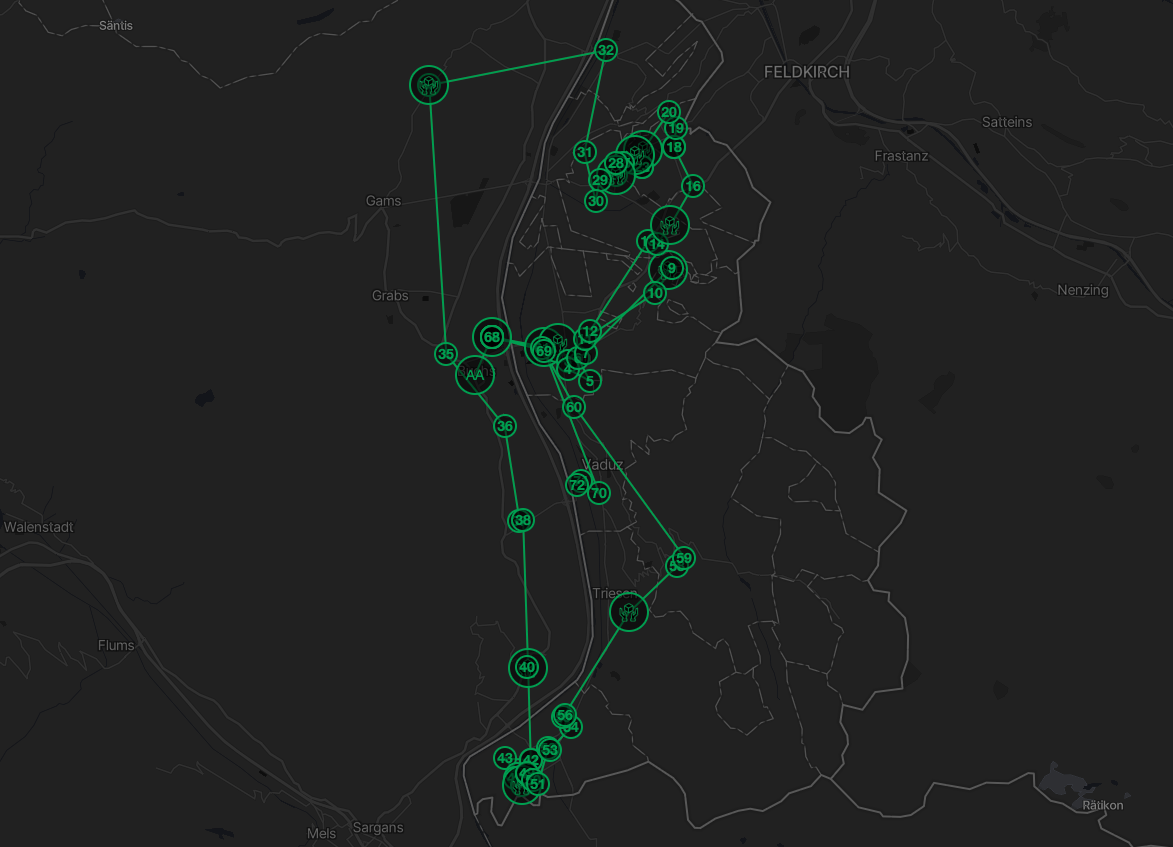
\includegraphics[width=0.75\textwidth]{resources/intro/hofkorb.png}
    \caption{Grocery delivery planning with multiple depots from the GoDeliver system}
    \label{fig:hofkorb}
\end{figure}

At GoDeliver, we are building an autonomous last-mile delivery system and at the core is a planning system which is solving various \gls{vrp}. The flavour which we are focusing on is Dynamic Capacitated Vehicle Routing Problem with Time Windows and Pick and Delivery (CVRPDPTW). GoDeliver typical use case is on-demand food delivery with multiple depots (pick and deliver), this means that the system has to be dynamic and flexible because a new customers are ordering stochastically for a chosen time window. Another our common use case shown in \ref{fig:hofkorb} is grocery delivery with multiple depots, time windows, and capacity for customers.
